
\documentclass[12pt,leqno]{article}

\usepackage{graphicx,color,amsmath,amsfonts,amssymb,amscd,amsthm,amsbsy,upref}


\textheight=8.5truein
\textwidth=6.0truein
\hoffset=-.5truein
\voffset=-.5truein
\numberwithin{equation}{section}
\pagestyle{headings}
\footskip=36pt

\newcommand{\question}[2] {\vspace{.25in} \noindent\fbox{#1} #2 \vspace{.10in}}

\swapnumbers
\theoremstyle{definition}
\newtheorem{thm}{Theorem}[section]
\newtheorem{hthm}[thm]{*Theorem}
\newtheorem{lem}[thm]{Lemma}
\newtheorem{cor}[thm]{Corollary}
\newtheorem{prop}[thm]{Proposition}
\newtheorem{con}[thm]{Conjecture}
\newtheorem{exer}[thm]{Exercise}
\newtheorem{bpe}[thm]{Blank Paper Exercise}
\newtheorem{apex}[thm]{Applications Exercise}
\newtheorem{ques}[thm]{Question}
\newtheorem{scho}[thm]{Scholium}
\newtheorem*{Exthm}{Example Theorem}
\newtheorem*{Thm}{Theorem}
\newtheorem*{Con}{Conjecture}
\newtheorem*{Axiom}{Axiom}

\newtheorem*{Ex}{Example}
\newtheorem*{Def}{Definition}
\newtheorem*{Lem}{Lemma}

\newcommand{\lcm}{\operatorname{lcm}}
\newcommand{\ord}{\operatorname{ord}}
\def\pfrac#1#2{{\left(\frac{#1}{#2}\right)}}


\makeindex

\begin{document}


\thispagestyle{plain}
\begin{flushright}
\large{\textbf{Khalid Hourani\\
}}
\end{flushright}

\question{2}{Prove that a subgroup of a solvable group is solvable.}

\begin{Thm}
 Let $G$ be a solvable group. Then every subgroup of $G$ is solvable.
\end{Thm}

\begin{proof}
 Take $H\leq G$. Since $G$ is solvable, $G^{(k)}=\{e\}$ for some $k$. Observe that, since $H\leq G$, $H'\leq G'$. Then, for all $i\leq k$, $H^{(i)}\leq G^{(i)}$. Hence, $H^{(k)}\leq G^{(k)}=\{e\}$, so $H$ is solvable.  
\end{proof}

\question{5}{If $N$ is a normal subgroup of $G$ prove that $N'$ must also be a normal subgroup of $G$.}

\begin{Thm}
 Let $G$ be a group and $N$ a normal subgroup of $G$. Then $N'\triangleleft G$.
\end{Thm}

\begin{proof}
 Take $n\in N'$, i.e. $n=xyx^{-1}y^{-1}$ for some $x,y\in N$. Then, for any $g\in G$, \begin{align*}gng^{-1}&=gxyx^{-1}y^{-1}g^{-1}\\&=(gxg^{-1})(gyg^{-1})(gx^{-1}g^{-1})(gy^{-1}g^{-1})\end{align*} Letting $u=gxg^{-1}$ and $v=gyg^{-1}$, we see that $u,v\in N$, for $N$ is normal in $G$. Hence, \[gng^{-1}=uvu^{-1}v^{-1}\in N'\qedhere\]
\end{proof}

\question{4}{Prove that any transposition and $p$-cycle generate $S_p$, with $p$ a prime.}


\question{5}{Show that the following polynomials of $\mathbb{Q}$ are irreducible and have exactly 2 non-real roots.}
\begin{description}
 \item [(a)] $p(x)=x^3-3x-3$
 \item [(b)] $p(x)=x^5-6x+3$
 \item [(c)] $p(x)=x^5+5x^4+10x^3+10x^2-x-2$
\end{description}

\pagebreak\begin{proof}[Solution]
 \begin{description}
  \item [(a)] Observe that $3$ does not divide $1$, $3$ divides $-3$ and $3^2=9$ does not divide $-3$. By the Eisenstein Criterion, $x^3-3x-3$ is irreducible over the rationals. The graph of $x^3-3x-3$ is 
\begin{figure*}[h]
\centering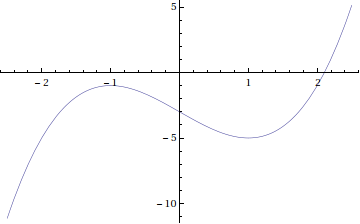
\includegraphics[scale=.5]{5-5-a.png}                                                                                                                                                                                                                                                                                                                                                               \end{figure*}

which shows that there is exactly one real root. Hence, the remaining two roots are non-real. 
  \item [(b)] Observe that $3$ does not divide $1$, $3$ divides $-6|$, $3|3$ and $3^2=9$ does not divide $3$. By the Eisenstein Criterion, $x^5-6x+3$ is irreducible over the rationals. The graph of $x^3-3x-3$ is
\begin{figure*}[h]
\centering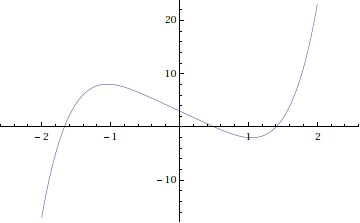
\includegraphics[scale=.5]{5-5-b.png}                                                                                                                                                                                                                                                                                                                                                               \end{figure*} 

which shows that there are exactly three real roots. Hence, the remaining two roots are non-real.
  \item [(c)] $x^5+5x^4+10x^3+10x^2-x-2$ has graph 
\begin{figure*}[h]
\centering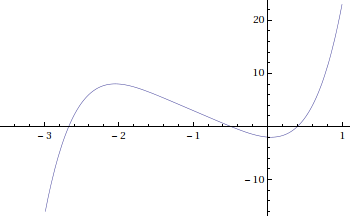
\includegraphics[scale=.5]{5-5-c.png}                                                                                                                                                                                                                                                                                                                                                               \end{figure*} 

which shows that there are exactly three real roots. Hence, the remaining two roots are non-real.
 \end{description}

\end{proof}

\question{6}{What are the Galois groups over $\mathbb{Q}$ of the polynomials in problem 5?}

\begin{proof}[Solution]
 Since these polynomials are irreducible of prime degree with exactly two non-real roots, it follows that their Galois groups are $S_3,S_5$ and $S_5$, respectively.
\end{proof}

\question{7}{Construct a polynomial of degree 7 with rational coefficients whose Galois group over $\mathbb{Q}$ is $S_7$.}

\begin{proof}[Solution]
 Consider $p(x)=x^7-4x^6+8x^4-2$. This polynomial satisfies Eisenstein's Criterion for $n=2$, so it is irreducible. Further, it has exactly 5 real roots and therefore exactly 2 non-real roots, and so the Galois group of $x^7-4x^6+8x^4-2$ over $\mathbb{Q}$ is $S_7$. 
\end{proof}

\end{document}
